\begin{figure*}[!t]
    \centering
    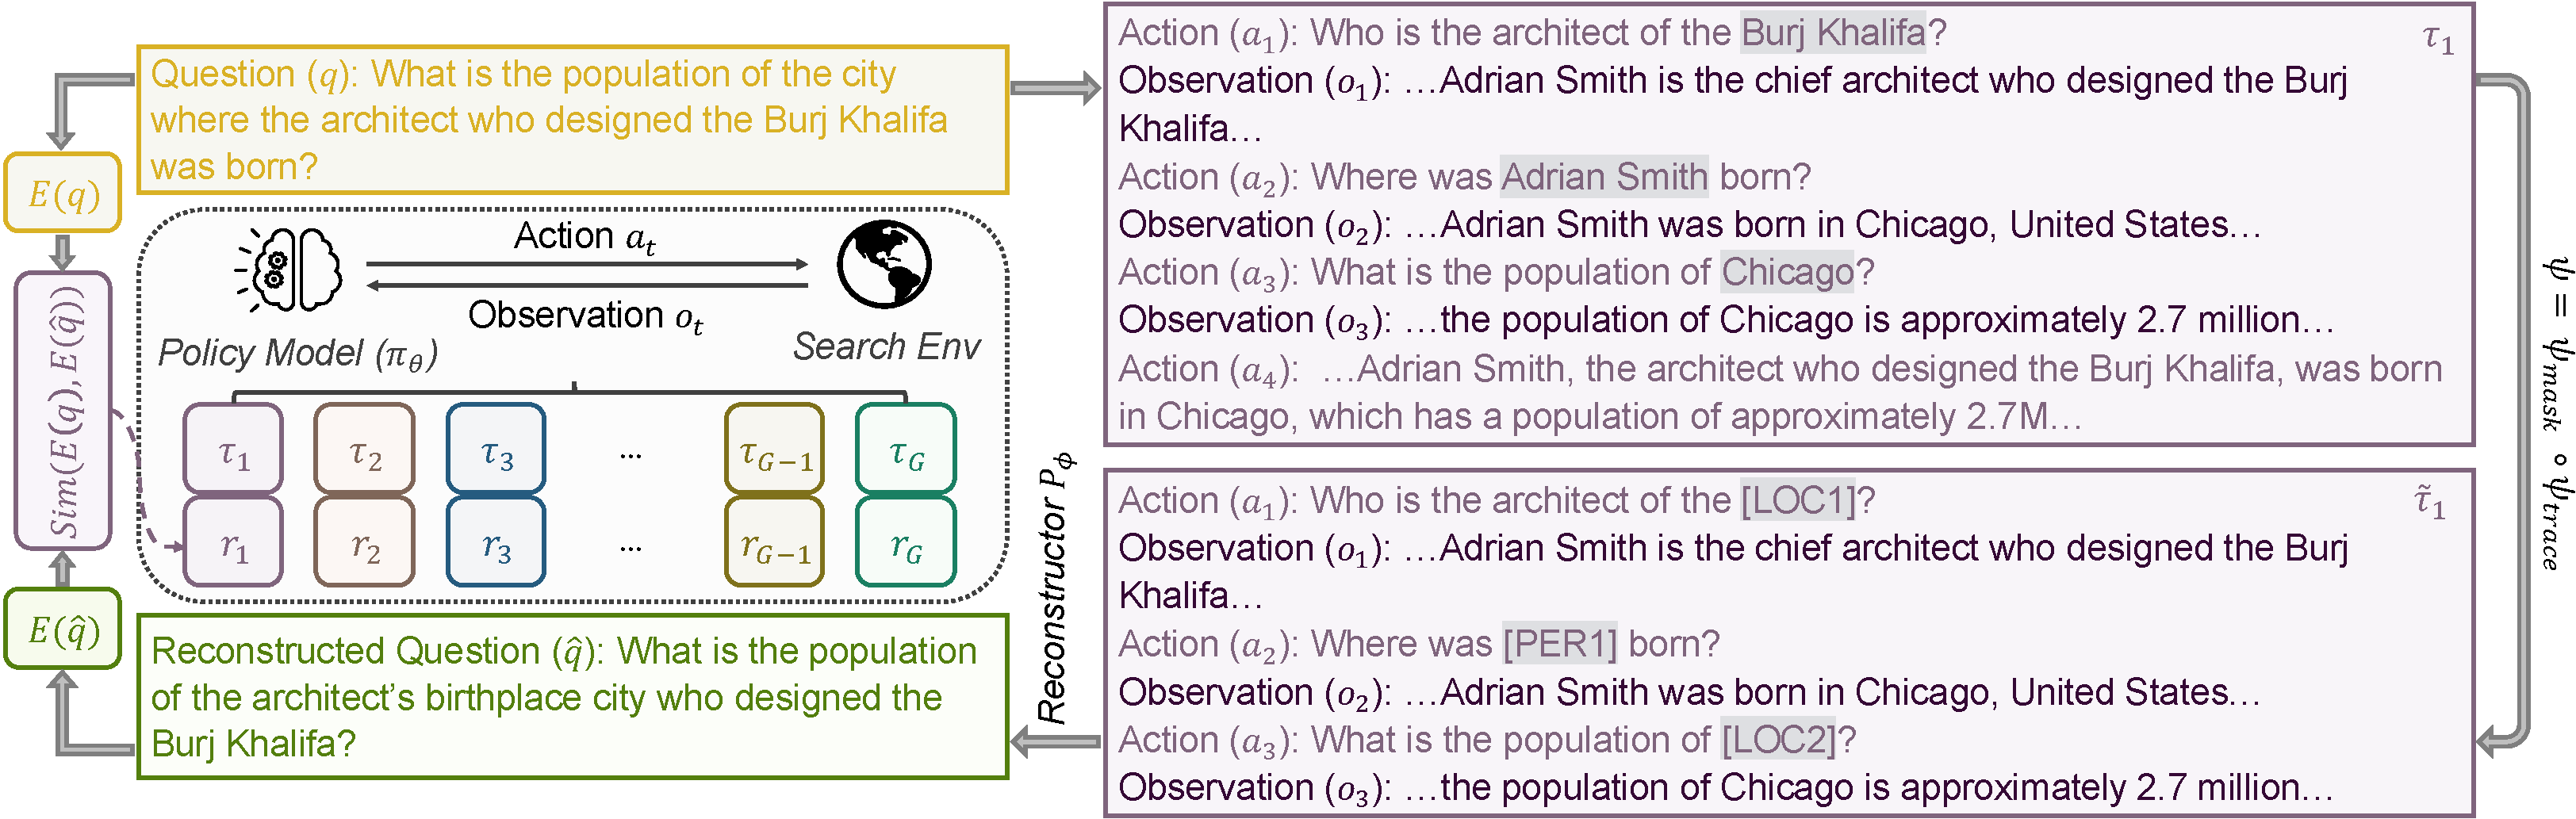
\includegraphics[width=1\linewidth]{img/ccs_main.pdf}
    \caption{\textbf{Overview of the Cycle-Consistent Search (CCS) framework.} The agent $\pi_\theta$ generates search trajectories $\tau$ to address a question $q$. To ensure the search process is driven by information gain rather than lexical copying, $\tau$ is passed through a strategic information bottleneck ($\psi$) that removes the $a_T$ and masks entities within actions (highlighted in grey). A frozen reconstructor $P_\phi$ then attempts to recover the original question from $\tilde{\tau}$. The agent is optimized using GRPO based on the semantic similarity between $q$ and $\hat{q}$, encouraging trajectories that capture sufficient evidence.}
    \label{fig:ccs_main}
\end{figure*}

% \vspace{-0.1in}

\section{Method}
% \vspace{-0.1in}
In this section, we formally introduce \textbf{Cycle-Consistent Search (CCS)}, a framework designed to train search agents \emph{without gold supervision}. We first establish the theoretical connection between search trajectory optimization and cycle-consistency. We then derive an information-theoretic objective and introduce structural constraints that prevent information leakage. Finally, we detail the optimization procedure using Group Relative Policy Optimization (GRPO). A schematic overview of CCS is shown in \Cref{fig:ccs_main}.

% \vspace{-0.1in}
\subsection{Cycle-Consistency as Information Conservation}
\label{sec:cycle-consistency}
% \vspace{-0.1in}
Our approach is grounded in the principle of cycle-consistency, widely utilized in unsupervised machine translation \citep{he2016dual, lample2017unsupervised, han2021unsupervised} and unpaired image-to-image translation \citep{cyclegan, liu2017unsupervised, huang2018multimodal}. Let $\mathcal{X}$ and $\mathcal{Y}$ denote two distinct domains. The fundamental assumption in these settings is that an ideal mapping $F: \mathcal{X}\rightarrow \mathcal{Y}$ preserves the essential semantic content of the input, such that there exists an inverse mapping $G:\mathcal{Y}\rightarrow \mathcal{X}$ satisfying $x \approx G(F(x))$ for any $x\in\mathcal{X}$. This implies that the transformation is information-preserving: the latent information required to reconstruct $x$ is conserved throughout the transformation.

We transpose this principle to agentic search. A user's question $q\in\mathcal{Q}$ represents a semantic intent, and a search trajectory $\tau\in\mathcal{T}$ represents a dynamic expansion of that intent into a sequence of actions and observations. Under the assumption of information conservation, an optimal search trajectory $\tau^*$ acts as a \emph{lossless encoding} of the question $q$. Consequently, if $\tau$ contains the necessary and sufficient evidence to resolve $q$, it should be possible to reconstruct $q$ solely from $\tau$. Formally, this establishes a cycle $q \rightarrow \tau \rightarrow \hat{q}$, where the closeness between $q$ and $\hat{q}$ serves as a proxy for the quality of the intermediate representation $\tau$, independent of external supervision.

% \vspace{-0.1in}
\subsection{Problem Formulation and Objective}
\label{sec:problem_formulation}
% \vspace{-0.1in}
We model the search process as a Partially Observable Markov Decision Process (POMDP). The agent, parameterized by $\theta$, is defined as a policy $\pi_\theta(\cdot \mid q, h_{t-1})$, where $h_{t-1}$ is the history of past actions and observations. At each intermediate step $t<T$, the agent issues an \emph{action} (search query) $a_t$ and receives an \emph{observation} (search results) $o_t$ from the search environment. After $T-1$ search steps, the agent produces a \emph{final response} $a_T$. The full trajectory is $\tau = (a_1, o_1, \ldots, a_{T-1}, o_{T-1}, a_T)$.

Under the cycle-consistency view in \Cref{sec:cycle-consistency}, the training objective can be formulated as maximizing the mutual information (MI) between the original question $q$ and the generated trajectory $\tau$.
Here, the mutual information $I(Q; \mathcal{T}_\theta)$ is defined as:
\begin{equation}
    I(Q; \mathcal{T}_\theta) = H(Q) - H(Q \mid \mathcal{T}_\theta).
\end{equation}
Since the entropy of the question distribution $H(Q)$ is constant with respect to $\theta$, maximizing MI is equivalent to minimizing the conditional entropy $H(Q \mid \mathcal{T}_\theta)$, which corresponds to maximizing the expected log-likelihood of the question given the trajectory:
\begin{equation}
    \mathcal{J}(\theta) = \mathbb{E}_{q \sim \mathcal{D}, \tau \sim \pi_\theta(\cdot\mid q)} \left[ \log P(q \mid \tau) \right].
\end{equation}
Directly modeling the true posterior $P(q \mid \tau)$ is intractable. We therefore employ a variational surrogate using a fixed, pre-trained reconstructor $P_\phi(q \mid \cdot)$, which serves as a tractable approximation to the inverse mapping $G$.

However, naively maximizing $\log P_\phi(q\mid\tau)$ can lead to degenerate solutions in which the agent encodes $q$ into the action sequence through trivial lexical copying (e.g., by repeating the question in a search query or partially restating it in the final response for context), allowing the reconstructor to recover $q$ without relying on the search results. To mitigate this issue, we introduce a bottleneck transformation $\psi: \mathcal{T} \rightarrow \tilde{\mathcal{T}}$ and optimize the following objective:
\begin{equation}
    \theta^* = \operatorname*{argmax}_\theta
    \mathbb{E}_{q \sim \mathcal{D},\, \tau \sim \pi_\theta(\cdot\mid q)}
    \left[ \log P_\phi\big(q \mid \psi(\tau)\big) \right].
\end{equation}

\subsection{Strategic Information Bottlenecks}
% \vspace{-0.1in}
The transformation function $\psi$ imposes structural constraints on the trajectory so that it retains the search scaffold while reducing lexical shortcuts that would otherwise allow trivial reconstruction of the source question.
We define $\psi$ as the composition of two operations: \emph{final response exclusion} and \emph{entity masking}: $\psi = \psi_{\text{mask}} \circ \psi_{\text{trace}}$.

% \vspace{-0.1in}
\paragraph{Final response exclusion.}
We first address leakage through the final response. In standard QA interactions, the final response $a_T$ often paraphrases $q$ to provide context. Including it in the reconstruction input can bypass the evaluation of the search process. Therefore, we define the trace operator $\psi_{\text{trace}}$ which truncates the trajectory to exclude the final generation step, preserving only the investigative actions and observations: $\psi_{\text{trace}}(\tau) = (a_1, o_1, \ldots, a_{T-1}, o_{T-1})$.

% \vspace{-0.1in}
\paragraph{Entity masking on search actions.}
We next mitigate leakage through search queries. Raw search queries $a_t$ typically exhibit high lexical overlap with $q$. To prevent the reconstructor from recovering $q$ from these surface-level cues even when the underlying search process is uninformative, we apply a masking operator $\psi_{\text{mask}}$ that identifies named entities within each search query $a_t$ (e.g., ``Burj Khalifa'') and replaces them with generic typed tags (e.g., \texttt{[LOC]}), yielding a masked action $\tilde{a}_t$. The observations $o_t$ remain unmasked. This operation substantially reduces the direct lexical channel from actions to the question, forcing reconstruction to resolve masked content primarily from evidence in $o_t$ rather than from copied words in $a_t$.

The full bottleneck transformation produces a processed trajectory: $\psi(\tau) = \tilde{\tau} = (\tilde{a}_1, o_1, \ldots, \tilde{a}_{T-1}, o_{T-1})$.
Consequently, to recover the original question from $\tilde{\tau}$, the reconstructor must leverage the information in the observations together with the structural intent expressed by the masked queries (e.g., $\tilde{\tau}_1$ in \Cref{fig:ccs_main}).
Trajectories with an incorrect or insufficient search scaffold, or with irrelevant or insufficient observations, will fail to preserve the relational structure or informational content required to reconstruct the original question, resulting in low reconstruction fidelity and thus low reward.
By tying the agent's incentive to both the correctness of the search scaffold and the informativeness of the resulting observations, CCS makes the reward sensitive to the quality of the search trajectory. In this way, the cycle-consistency objective penalizes trajectories that are incorrect, incomplete, or noisy, while favoring those that preserve the relational structure of the question and gather the information required for faithful reconstruction.


\subsection{Optimization via Group Relative Policy Optimization}
% \vspace{-0.1in}
The objective in \Cref{sec:problem_formulation} frames search-agent training as maximizing the reconstructability of the original question from the bottlenecked trajectory. This naturally defines a trajectory-level reward: trajectories that better preserve the information needed to reconstruct $q$ receive higher rewards.
We optimize the search agent with reinforcement learning using our cycle-consistency reward. Specifically, we adopt Group Relative Policy Optimization (GRPO) \citep{grpo}, which has proven effective for search-agent optimization \citep{search-r1} and avoids the need for a separate value-function critic by using group-based relative advantages.

The RL objective is to optimize $\pi_\theta$ by maximizing expected returns over questions $q\sim\mathcal{D}$:
\begin{equation}
    \max_{\pi_\theta} \mathbb{E}_{q \sim \mathcal{D}, \tau \sim \pi_\theta(\cdot\mid q)} \big[r(\tau)\big].
\end{equation}
For each question $q$, the agent samples a group of $G$ trajectories $\{\tau_1,\tau_2,\dots,\tau_G\}$ from the current policy $\pi_{\theta_{\text{old}}}$. For each $\tau_i$, we compute a reconstructed question $\hat{q}_i \sim P_\phi(\cdot \mid \psi(\tau_i))$ and define the reward as the semantic similarity between $q$ and $\hat{q}_i$:
\begin{equation}
    r(\tau_i) = \mathrm{Sim}\big(E(q), E(\hat{q}_i)\big),
    \label{eq:embedding_sim}
\end{equation}
where $E(\cdot)$ is a sentence embedding function and $\mathrm{Sim}(\cdot,\cdot)$ denotes cosine similarity.

We then compute an advantage $A_i$ by normalizing rewards within the group:
\begin{equation}
    A_i = \frac{r(\tau_i) - \mu(\{r(\tau_j)\}_{j=1}^G)}{\sigma(\{r(\tau_j)\}_{j=1}^G) + \epsilon},
\end{equation}
where $\mu$ and $\sigma$ denote the mean and standard deviation of group rewards. The GRPO objective is then:
\begin{equation}
\begin{aligned}
\mathcal{L}_{GRPO}(\theta)
= \mathbb{E}_{q \sim \mathcal{D}} \Bigg[
\frac{1}{G} \sum_{i=1}^G
\Big(
\min \Big(
\frac{\pi_\theta(\tau_i|q)}{\pi_{\theta_{old}}(\tau_i|q)} A_i,
\text{clip}\Big(
\frac{\pi_\theta(\tau_i|q)}{\pi_{\theta_{old}}(\tau_i|q)},
1-\epsilon, 1+\epsilon
\Big) A_i
\Big)
\\
- \beta \mathbb{D}_{KL}(\pi_\theta \,\|\, \pi_{ref})
\Big)
\Bigg].
\end{aligned}
\end{equation}
Here, observations are treated as environment outputs and $\pi_\theta(\tau_i\mid q)$ refers to the likelihood of the agent-generated tokens/actions \citep{search-r1}.
This objective increases the likelihood of trajectories that yield higher reconstruction fidelity relative to the group average, thereby encouraging search behaviors that better preserve the structure and information needed to recover the original question.